\documentclass{beamer}
\usepackage{beamer}
\usepackage{amsthm,amsmath,amssymb,mathrsfs, dsfont}
\usepackage[english]{babel}
\usepackage[T1]{fontenc}
\usepackage[utf8]{inputenc}
\usepackage{amsmath}
\usepackage{ragged2e}
\usepackage{xcolor}
\colorlet{shaded}{gray!40} 

\usepackage{graphicx}
\usepackage{tikz}
\usetikzlibrary{shapes.geometric}
\usetikzlibrary{arrows.meta,arrows}
\usepackage[draft]{tikzit}
\input{hypergraph.tikzdefs}
\input{hypergraph.tikzstyles}
\usetikzlibrary{decorations.markings}
\usepackage[all, cmtip]{xy}
\usepackage{svg}

%%% Bibliography
\usepackage[style=numeric,backend=bibtex]{biblatex}
\addbibresource{biblio.bib}
\renewcommand*{\bibfont}{\footnotesize}

% default color is dark

\def\colortheme{dark} % preset themes available are lighten, light, dark
\def\alertcolor{dark} % preset themes available are lighten, light, dark
\def\upperbar{\true} % i want upper index/navigation bar, \true or \false
\def\bottomsectionbar{\true} % i want bottom bar with Title and Frame/Slide number, \true or \false
\def\bottomtitlebar{\false} % i want bottom bar with Section and Institute, \true or \false

% % %
\if\upperbar\false
    \setbeamertemplate{headline}{}
\fi
% % %


\newcommand{\catname}[1]{\textbf{\textup{#1}}}
\newcommand{\tg}[0]{\catname{TG}_{\Sigma}}
\newcommand{\eg}{\catname{EGG}}
\newcommand{\egg}{\mathsf{e}\text{-}\catname{EqHyp}}
\newcommand{\hyp}{\catname{Hyp}}
\newcommand{\hyps}{\catname{Hyp}_{\Sigma}}
\newcommand{\EqHyp}{\catname{EqHyp}} %equivalence hypergraphs
\newcommand{\EqHyps}{\catname{EqHyp}_{\Sigma}}
\newcommand{\EqTG}{\catname{EqTG}}
\newcommand{\EqTGs}{\catname{EqTG}_{\Sigma}}
\newcommand{\eto}{\twoheadrightarrow}
\newcommand{\mto}{\rightarrowtail}


\newcommand{\pbc}{\mathsf{Pb}}
\newcommand{\pbe}{\mathsf{ePb}}

\title{EGGs are adhesive!}
%\subtitle{Subtitle}
\author{R. Biondo, \textbf{D. Castelnovo} and F. Gadducci}
\institute
{
  University of Pisa
}
\date{Glasgow, \today}

\def\X{\textbf {\textup{X}}}
\def\Y{\textbf {\textup{Y}}}
\def\D{\textbf {\textup{D}}}

\newenvironment{noheadlineframe}
{%
	\setbeamertemplate{headline}{}%
	\begin{frame}
	}
	{%
	\end{frame}
}

\begin{document}

\firstpage % optional. First page

%\indexoverview % optional. Make a slide with index 

\section{Intro: EGGs}\justifying

%\sectionoverview % optional. Make a slide with section structure index 

\begin{frame}{What are EGGs?} % normal itemize, one frame
    
    \emph{e-graphs (EGGS)} \cite{DetlefsNS05,WillseyNWFTP21} are a graphical formalism  for program optimisation  via an efficient implementation of equality saturation. 
    
    \pause \medskip 
    
     They can be  defined as (acyclic) term graphs \cite{corradini2005term,Plu:TGR-ENTCS} with an additional notion of  equivalence on nodes that is closed under the operators of the signature.
     
     \pause \medskip The idea is that nodes representing the same term should be in the same equivalence class. \pause 
     
     
     \begin{center}
     	\hspace{.25cm}
     		\begin{tikzpicture}[baseline=(nil.center)]\begin{pgfonlayer}{nodelayer}
     				\node[style=node](v1) at (-0.9, 0.3){};
     				\node[style=node](v2) at (-0.9, -0.3){};
     				\node[style=medium box] at (0, 0){$/$};
     				\node[style=none](divfst) at (-0.3, 0.3){};
     				\node[style=none](divsnd) at (-0.3, -0.3){};
     				\node[style=none](divout) at (0.3, 0){};
     				\node[style=node] (w) at (0.9, 0){};
     				\node[style=small box] at (0, -1){$1$};
     				\node[style=none](one) at (0.3, -1){};
     				\node[style=node](z) at (0.9, -1){};
     				\node[style=none](nil) at (0, -0.5){};
     			\end{pgfonlayer}        
     			\begin{pgfonlayer}{edgelayer}
     				\draw(v1) to (divfst.center);
     				\draw(v2) to (divsnd.center);
     				\draw(divout.center) to (w);
     				\draw(one.center) to (z);
     			\end{pgfonlayer}
     			\begin{pgfonlayer}{eqlayer}
     				\draw[dashed, rounded corners](-1.2, 0.6) rectangle (-0.6, -0.6);
     				\draw[dashed, rounded corners](0.6, 0.3) rectangle (1.2, -1.3);
     			\end{pgfonlayer}\begin{pgfonlayer}{background}
     				\draw[color=white] (-1.5, 0.2) rectangle (1.5, -0.2);
     		\end{pgfonlayer}\end{tikzpicture}
     \end{center}
\end{frame}


\begin{frame}{Aims of this work} 
    \begin{itemize}
        \item Formalize the definition of EGGs in a categorical setting and study their properties. \pause \medskip 
        \item Develop the theory of EGGs rewriting using the Double Pushout (DPO) paradigm \cite{ehrig2006fundamentals,ehrig1999handbook}.
    \end{itemize}
\end{frame}

\section{DPO rewriting}

\begin{frame}{DPO rewriting systems} 
	\begin{overprint}

		\onslide<1|handout:1>
		
		A \emph{DPO-rewriting rule} is a pair of arrows $l:K\to L$ and $r:K\to R$ with the same domain. To rewrite an object $G$ according to a rule we proceed in three steps.
		
		\onslide<2| handout:0>
		
	A \emph{DPO-rewriting rule} is a pair  of arrows $l:K\to L$ and $r:K\to R$ with the same domain. To rewrite an object $G$ according to a rule we proceed in three steps.
		
		\medskip
		First: find a \emph{match} $m:L\to G$.
		\begin{center}
			\begin{tikzpicture}
				\node(L)at(0,0){$L$};
				\node(K)at(2,0){$K$};
				\node(R)at(4,0){$R$};
				\node(G)at(0,-2){$G$};
				\draw[->](K)--(L)node[pos=0.5, above]{$l$};
				\draw[->](K)--(R)node[pos=0.5, above]{$r$};
				\draw[->, dotted](L)--(G)node[pos=0.5, left]{$m$};
			\end{tikzpicture}
		\end{center}
		
		
		\onslide<3| handout:0>
		
		A \emph{DPO-rewriting rule} is a pair  of arrows $l:K\to L$ and $r:K\to R$ with the same domain. To rewrite an object $G$ according to a rule we proceed in three steps.		
		
		\medskip
		Second: ``remove'' the image of $m$  building a pushout square. \vspace{-0.075cm}
		\begin{center}
			\begin{tikzpicture}
				\node(L)at(0,0){$L$};
				\node(K)at(2,0){$K$};
				\node(R)at(4,0){$R$};
				\node(G)at(0,-2){$G$};
				\node(C)at(2,-2){$C$};
				\draw[->](K)--(L)node[pos=0.5, above]{$l$};
				\draw[->](K)--(R)node[pos=0.5, above]{$r$};
				\draw[->](L)--(G)node[pos=0.5, left]{$m$};
				\draw[->, dotted](K)--(C)node[pos=0.5, right]{$p$};
				\draw[->, dotted](C)--(G)node[pos=0.5, below]{$l'$};
			\end{tikzpicture}
		\end{center}		
		\onslide<4| handout:0>
		
	A \emph{DPO-rewriting rule} is a pair  of arrows $l:K\to L$ and $r:K\to R$ with the same domain. To rewrite an object $G$ according to a rule we proceed in three steps.
		
		\medskip
		Third: glue $R$ into the ``hole'',  taking a pushout.\vspace{-0.075cm}
		\begin{center}\hspace{0.08cm}
			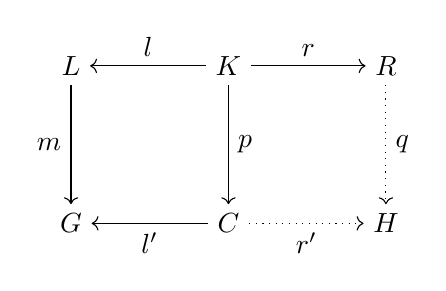
\begin{tikzpicture}
				\node(L)at(0,0){$L$};
				\node(K)at(2,0){$K$};
				\node(R)at(4,0){$R$};
				\node(G)at(0,-2){$G$};
				\node(C)at(2,-2){$C$};
				\node(H)at(4,-2){$H$};
				\draw[->](K)--(L)node[pos=0.5, above]{$l$};
				\draw[->](K)--(R)node[pos=0.5, above]{$r$};
				\draw[->](L)--(G)node[pos=0.5, left]{$m$};
				\draw[->](K)--(C)node[pos=0.5, right]{$p$};
				\draw[->](C)--(G)node[pos=0.5, below]{$l'$};
				\draw[->, dotted ](C)--(H)node[pos=0.5, below]{$r'$};
				\draw[->, dotted ](R)--(H)node[pos=0.5, right]{$q$};
			\end{tikzpicture}
		\end{center}		
	\end{overprint}  	
\end{frame}




\begin{frame}{$\mathcal{M}$-adhesive categories}
	The categorical framework for DPO rewriting is given by \emph{$\mathcal{M}$-adhesive categories} \cite{azzi2019essence,ehrig2014adhesive, lack2005adhesive}.
		
		\medskip \pause
		Let $\mathcal{M}$ be a class of monos in a category $\X$, containing all isomorphisms, stable under pullbacks and composition. $\X$ is \emph{$\mathcal{M}$-adhesive} if, given a cube below with the hooked arrows in $\mathcal{M}$, the bottom face a pushout and the back faces pullbacks, we have:
		
		\parbox{5cm}{\centering 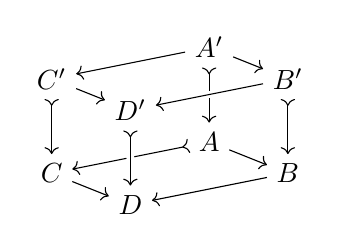
\begin{tikzpicture}
				\node(C)at(-1,0.4){$C$};
				\node(A)at(1,0.8){$A$};
				\node(B)at(2,0.4){$B$};
				\node(D)at(0,0){$D$};
				\node(A')at(1,2){$A'$};
				\node(B')at(2,1.6){$B'$};
				\node(C')at(-1,1.6){$C'$};
				\node(D')at(0,1.2){$D'$};
				\draw[<-](B')--(A');
				\draw[>->](B')--(B);
				\draw[>->](C')--(C); 
				\draw[>->](D')--(D);
				\draw[->](A')--(C'); 
				\draw[->](B')--(D');
				\draw[->](C')--(D');
				\draw[->](A)--(B);
				\draw[->](C)--(D);
				\draw[->](B)--(D);
				\draw[>-](A')--(1,1.45);
				\draw[->](1,1.35)--(A);
				\draw[>-](A)--(0.05, 0.61);
				\draw[<-](C)--(-0.05,0.59);
		\end{tikzpicture}} \quad 	\parbox{4cm}{\centering
			Top face is a pushout \\ $\iff$ \\ Front faces are pullbacks}
			

\end{frame}

\begin{frame}

$\mathcal{M}$-adhesivity is preserved by common categorical constructions:\pause
\begin{itemize}
	\item products\pause 
	\item functor categories \pause
	\item slices and coslices
\end{itemize}

\pause 

Moreover, a full subcategory closed under the relevant pullbacks and pushouts inherits the adhesivity properties of the bigger one.
\end{frame}


\section{Hypergraphical structures }


\begin{frame}{Hypergraphs}

A hypergraph is a 4-uple $(E, V, s, t)$ made by two sets $E$ and $V$ (\emph{edges} and \emph{nodes}) and arrows $s, t\colon E \rightrightarrows V^\star$. \pause A \emph{hypergraph morphism} $(E, V, s, t)\to (F, W, s,' t')$  is a pair of arrow $h\colon E\to E'$ and $k\colon V\to V'$ fitting in the digram below.
	
	\[\xymatrix{ E \ar[r]^{h}\ar[d]_{s}& F \ar[d]^{s'} & E \ar[r]^{k} \ar[d]_{t}& F\ar[d]^{t'}\\ V^\star\ar[r]_{k^\star}& W^\star & V^\star \ar[r]_{k^\star}&W^\star}\]
		
	\pause 
\begin{theorem}
	The category $\hyp$ of hypergraphs is adhesive.
\end{theorem}	

\end{frame}

\begin{frame}{Labelling  hypergraphs}
	
	\parbox{.5\linewidth}{Given an algebraic signature $\Sigma$ one can build an hypergraph $\mathcal{G}_\Sigma$ with a single node and edges corresponding with operations of $\Sigma$.} \hfill
		\begin{minipage}[r]{.4\linewidth}
			\begin{tikzpicture}
				\begin{pgfonlayer}{nodelayer}
					\node[style=node] (v) at (0, 0){};
					\node[style=none] (vlab) at (0, -0.4){$v$};
					
					\node[style=small box] (n) at (1.8, 0) {};
					\node[style=none] (nlab) at (2.4, 0.0) {$1$};
					\node[style=none] (nattach) at (1.6, 0) {};
					
					
					\node[style=medium box] (times) at (-1, 1.8) {};
					\node[style=none] (timeslab) at (-1, 2.6) {$\cdot$};
					\node[style=none] (timesin1) at (-1.2, 1.25) {};
					\node[style=none] (timesin2) at (-0.8, 1.25) {};
					\node[style=none] (timesout) at (-0.8, 1.8){};
					
					\node[style=medium box] (div) at (1, 1.8) {};
					\node[style=none] (divlab) at (1, 2.6) {$(-)^{-1}$};
					\node[style=none] (divin1) at (0.8, 1.25) {};
					\node[style=none] (divin2) at (1.2, 1.25) {};
					\node[style=none] (divout) at (0.8, 1.8){};
				\end{pgfonlayer}
				
				
				\begin{pgfonlayer}{edgelayer}
					\draw[style=diredge, in=270, out= 160] (v) to (timesin2.center); 
					\draw[style=diredge,out=200, in= 270] (v) to (timesin1.center);
					\draw[style=diredge,in=0, out=0] (nattach.center) to (v);
					
					\draw[style=diredge,in=270, out=20] (v) to (divin2.center); 
					\draw[style=diredge,out=60, in= 270] (v) to (divin1.center);
					
					\draw[style=diredge, in=120, out=0] (timesout.center) to (v);
					\draw[style=diredge, in=90, out=180] (divout.center) to (v);
				\end{pgfonlayer}
				
			\end{tikzpicture}
		\end{minipage}
	\pause 
	
	\medskip 
	The category $\hyp_{\Sigma}$ of \emph{labelled hypergraphs} is the slice $\hyp/\mathcal{G}_\Sigma$.
	
	\pause 
	\begin{theorem}
		 \hspace{1pt}$\hyp_\Sigma$ is adhesive.
	\end{theorem}	
\end{frame}

\begin{frame}{Term graphs}
A \emph{term graph} \cite{corradini2005term,corradini1997algebraic, Plu:TGR-ENTCS} is a labelled hypergraphs with injective target function. $\tg$ is be the full subcategory of $\hyp_{\Sigma}$ given by them.

\pause 
\begin{itemize}
	\item monos in $\tg$ are morphism which are injective on both edges and nodes;\pause 
	\item regular monos in $\tg$ are monos which preserves \emph{input nodes}, i.e.~nodes not in the image of the target functions.
\end{itemize}
\pause 

\begin{theorem}
$\tg$ is quasiadhesive.
\end{theorem}

\end{frame}


\begin{frame}
	
	Summing up:
	
	
	\[\xymatrix@R=15pt@C=15pt{ \color{shaded}\eg \ar@{^{(}->}@[shaded][r]^-{\color{shaded}Y_\Sigma} \ar@{^{(}->}@[shaded][d]_{\color{shaded}K_\Sigma} & \color{shaded}\egg_\Sigma \ar@{^{(}->}@[shaded][d]_{\color{shaded} Z_\Sigma} \ar@[shaded][r]^{\color{shaded}W_\Sigma}&\color{shaded} \egg \ar@{^{(}->}@[shaded][d]^{\color{shaded}I}\\ \color{shaded}\EqTG_{\Sigma} \ar@{^{(}->}@[shaded][r]^{\color{shaded}J_\Sigma}\ar@[shaded][d]_{\color{shaded}S_\Sigma}&\color{shaded} \EqHyp_\Sigma \ar@[shaded][r]^{\color{shaded}V_\Sigma} \ar@[shaded][d]_{\color{shaded}T_\Sigma}&\color{shaded} \EqHyp \ar@[shaded][d]^{\color{shaded}T}\\ \tg \ar@{^{(}->}[r]_{I_\Sigma}& \hyp_{\Sigma} \ar[r]_{U_\Sigma}  &\hyp}\]
	
\end{frame}


\section{Adding equivalences}

\begin{frame}{Hypergraphs with equivalence}

A \emph{(labelled) hypergraph/term graph} is a (labelled) hypergraph/term graph equipped with a surjection $q\colon V\eto Q$ from the set of nodes. \pause 

We get categories $\EqHyp$, $\EqHyps$ and  $\EqTG_{\Sigma}$ asking that the nodes part of a morpism induces a mrphism between the quotients. 
\[\xymatrix{V \ar@{>>}[d]_{q} \ar[r]^{k}& W \ar@{>>}[d]^p\\ Q \ar@{.>}[r]_{u} & P }\]

\pause 

\begin{block}{Remark}\justifying
$\EqHyps$ is actually the slice over $\mathcal{G}_\Sigma$ endowed with the only possible quotient from $1$. $ \EqTG_{\Sigma}$ is a full subcategory of $\EqHyps$.
\end{block}
\end{frame}


\begin{frame}{Limits and colimits in $\EqHyp$}
	Colimits are computed componentwise. If $(E_d, V_d, Q_d, s_d, t_d, q_d )$ is a diagram of hypergraphs with equivalence, then a colimit is given by $(E, V, Q, s, t, q)$, where $E$, $V$, $Q$ are the colimits of $\{E_d\}_{d\in \D}$, $\{V_d\}_{d\in \D}$, $\{Q_d\}_{d\in \D}$ and $s, t, q$ are the natural ones.
	
	\pause  \medskip 
	\begin{minipage}[l]{0.45\linewidth}
		Limits are more difficult. In the example on the right, the pullback of the underlying hypergraphs gives us the empty one. The pullback of quotients is the singleton.
	\end{minipage} \qquad 
\begin{minipage}[r]{0.6\linewidth}
	\xymatrix{
		 &
		\begin{tikzpicture}[baseline=(v.base)]\begin{pgfonlayer}{nodelayer}
				\node[style=node](v) at (0, 0){};
				\node[style=none] at(0, 0.5){$c$};
			\end{pgfonlayer}
			\begin{pgfonlayer}{eqlayer}\draw[dashed, rounded corners] (-0.3, -0.3) rectangle (0.3, 0.3);\end{pgfonlayer}
		\end{tikzpicture}  \ar@{>->}@(d,)[d]!<0ex,0ex> \\ 
		\begin{tikzpicture}[baseline=(v.base)]\begin{pgfonlayer}{nodelayer}
				\node[style=node](v)at(0, 0){};
				\node[style=none]at(0, 0.5){$b$};
			\end{pgfonlayer}
			\begin{pgfonlayer}{eqlayer}\draw[dashed, rounded corners] (-0.3, -0.3) rectangle (0.3, 0.3);\end{pgfonlayer}
		\end{tikzpicture}
		\ar@{>->}@(r,)@<-.5ex>[r] & 
		\begin{tikzpicture}[baseline=(v.base)]\begin{pgfonlayer}{nodelayer}
				\node[style=node](v)at(-0.5, 0){};
				\node[style=none]at(-0.5, 0.5){$b$};
				\node[style=node]at(0.5, 0){};
				\node[style=none]at(0.5, 0.5){$c$};
			\end{pgfonlayer}\begin{pgfonlayer}{eqlayer}
				\draw[dashed, rounded corners](-0.8, 0.3) rectangle (0.8, -0.3);
		\end{pgfonlayer}\end{tikzpicture}
		 }
	\end{minipage}
\end{frame}

\begin{frame}{Limits and colimits in $\EqHyp$}

Luckily in $\catname{Set}$ we can factor any arrow as a surjection followed by an injection. 

\pause 
General recipe for limits: \pause 

\begin{enumerate}
	\item compute the limit $(E, V, s,t)$ of the underlying hypergraphs; \pause 
	\item compute the limit $L$ of the family of quotients; \pause 
	\item factor the natural arrow $V\to L$ as $V\eto Q \mto L$; \pause 
	\item $(E, V, Q, s,t, q )$ is a colimit for the original diagram, where $q\colon V\eto Q$.
\end{enumerate}	
	
\end{frame}


\begin{frame}{Hypergraphs with equivalence - adhesivity}
	
Pushouts along regular monos in $\EqHyp$ are not stable. 

\begin{center}
	\xymatrix@C=10pt@R=6pt{
		&\emptyset \ar@{>->}[dd]|\hole \ar@{>->}[rr] \ar@{>->}@(dl,)[dl] &&
		\begin{tikzpicture}[baseline=(v.base)]\begin{pgfonlayer}{nodelayer}
				\node[style=node](v) at (0, 0){};
				\node[style=none] at(0, 0.5){$c$};
			\end{pgfonlayer}
			\begin{pgfonlayer}{eqlayer}\draw[dashed, rounded corners] (-0.3, -0.3) rectangle (0.3, 0.3);\end{pgfonlayer}
		\end{tikzpicture} \ar@{>->}[dd] \ar@{>->}@(dl,)[dl]!<6ex,0ex> \\
		\begin{tikzpicture}[baseline=(v.base)]\begin{pgfonlayer}{nodelayer}
				\node[style=node](v)at(0, 0){};
				\node[style=none]at(0, 0.5){$b$};
			\end{pgfonlayer}
			\begin{pgfonlayer}{eqlayer}\draw[dashed, rounded corners] (-0.3, -0.3) rectangle (0.3, 0.3);\end{pgfonlayer}
		\end{tikzpicture}
		\ar@{>->}[dd]\ar@{>->}[rr] & &
		\begin{tikzpicture}[baseline=(v.base)]\begin{pgfonlayer}{nodelayer}
				\node[style=node](v)at(-0.5, 0){};
				\node[style=none]at(-0.5, 0.5){$b$};
				\node[style=node]at(0.5, 0){};
				\node[style=none]at(0.5, 0.5){$c$};
			\end{pgfonlayer}\begin{pgfonlayer}{eqlayer}
				\draw[dashed, rounded corners](-0.8, 0.3) rectangle (0.8, -0.3);
		\end{pgfonlayer}\end{tikzpicture}
		\ar@<2ex>@{>->}[dd]\\&
		\begin{tikzpicture}[baseline=(v.base)]\begin{pgfonlayer}{nodelayer}
				\node[style=node](v)at(0, 0){};
				\node[style=none]at(0, 0.5){$a$};
			\end{pgfonlayer}
			\begin{pgfonlayer}{eqlayer}\draw[dashed, rounded corners] (-0.3, -0.3) rectangle (0.3, 0.3);\end{pgfonlayer}
		\end{tikzpicture}
		\ar@{>->}[rr]|\hole \ar@{>->}@(dl,)[dl] && 
		\begin{tikzpicture}[baseline=(v.base)]\begin{pgfonlayer}{nodelayer}
				\node[style=node](v)at(-0.5, 0){};
				\node[style=none]at(-0.5, 0.5){$a$};
				\node[style=node]at(0.5, 0){};
				\node[style=none]at(0.5, 0.5){$c$};
			\end{pgfonlayer}\begin{pgfonlayer}{eqlayer}
				\draw[dashed, rounded corners](-0.8, 0.3) rectangle (0.8, -0.3);
		\end{pgfonlayer}\end{tikzpicture}
		\ar@{>->}@(,r)[dl] \\
		\begin{tikzpicture}[baseline=(v.base)]\begin{pgfonlayer}{nodelayer}
				\node[style=node](v)at(-0.5, 0){};
				\node[style=none]at(-0.5, 0.5){$a$};
				\node[style=node]at(0.5, 0){};
				\node[style=none]at(0.5, 0.5){$b$};
			\end{pgfonlayer}\begin{pgfonlayer}{eqlayer}
				\draw[dashed, rounded corners](-0.8, 0.3) rectangle (0.8, -0.3);
		\end{pgfonlayer}\end{tikzpicture}
		\ar@{>->}[rr] & & 
		\begin{tikzpicture}[baseline=(v.base)]\begin{pgfonlayer}{nodelayer}
				\node[style=node](v)at(0, 0){};
				\node[style=none]at(0, 0.5){$a$};
				\node[style=node]at(1, 0){};
				\node[style=none]at(1, 0.5){$b$};
				\node[style=node]at(2, 0){};
				\node[style=none]at(2, 0.5){$c$};
			\end{pgfonlayer}\begin{pgfonlayer}{eqlayer}
				\draw[dashed, rounded corners](-.3, 0.3) rectangle (2.3, -0.3);
	\end{pgfonlayer}\end{tikzpicture} }
\end{center}
\end{frame}



\begin{frame}{Hypergraphs with equivalence - adhesivity}
	\begin{minipage}[l]{.6\linewidth}
		We can find another class to test for adhesivity. Let $\pbc$ be the class of monos of $\EqHyp$ such that the square aside is a pullback.
	\end{minipage}\qquad 
	\begin{minipage}{.3\linewidth}
	\xymatrix{V \ar@{>>}[d]_{q} \ar@{>->}[r]^{k}& W \ar@{>>}[d]^p\\ Q \ar@{>->}[r]_{u} & P }
	\end{minipage}
	\pause 
	
	\begin{theorem}
		$\EqHyp$ is $\pbc$-adhesive.
	\end{theorem}
\end{frame}

\begin{frame}{Adhesivity of $\EqHyp_\Sigma$ and $\EqTG_{\Sigma}$}
	In the same way can define a labelled analog $\pbc_\Sigma$ of $\pbc$.
	\pause 
	\begin{theorem}
		$\EqHyp_\Sigma$ is $\pbc_\Sigma$-adhesive.
	\end{theorem} 
	
	\pause 
	For term graph, we can consider the class $\mathcal{T}$ of arrows which are in $\pbc_\Sigma$ and whose underlying term graph morphism is a regular mono.
	
	\pause 
	\begin{theorem}
		$\EqTG_{\Sigma}$ is $\mathcal{T}$-adhesive.
	\end{theorem}
	
	
\end{frame}



\begin{frame}
	
	Summing up:
	
	
	\[\xymatrix@R=15pt@C=15pt{ \color{shaded}\eg \ar@{^{(}->}@[shaded][r]^-{\color{shaded}Y_\Sigma} \ar@{^{(}->}@[shaded][d]_{\color{shaded}K_\Sigma} & \color{shaded}\egg_\Sigma \ar@{^{(}->}@[shaded][d]_{\color{shaded} Z_\Sigma} \ar@[shaded][r]^{\color{shaded}W_\Sigma}&\color{shaded} \egg \ar@{^{(}->}@[shaded][d]^{\color{shaded}I}\\ \EqTG_{\Sigma} \ar@{^{(}->}[r]^{J_\Sigma}\ar[d]_{S_\Sigma}& \EqHyp_\Sigma \ar[r]^{V_\Sigma} \ar[d]_{T_\Sigma}& \EqHyp \ar[d]^{T}\\ \tg \ar@{^{(}->}[r]_{I_\Sigma}& \hyp_{\Sigma} \ar[r]_{U_\Sigma}  &\hyp}\]
	
\end{frame}

\section{Congruences}


\begin{frame}{Congruences}

General equivalence relations are not enough. We want to restrict our attention to \emph{congruences}: whenever the relation identifies the source of two hyperedges, it identifies their targets too. 
	
\pause 

\begin{definition}\justifying 
	Let $\mathcal{G} = (E, V, Q, s, t, q)$ be a hypergraph with equivalence and $(S, \pi_1, \pi_2)$ a kernel pair for $q^\star \circ s$.
We will say that $\mathcal{G}$ is an \emph{e-hypergraph} if $q^\star \circ t \circ \pi_1 = q^\star \circ t \circ \pi_2$.
\end{definition}	
	
	\pause 
	Restricting to e-hypergraphs we get: \pause 
\begin{itemize}\justifying
	\item $\egg$: full subcategory of e-hypergraphs; \pause 
	\item $\egg_\Sigma$: the subcategory of $\EqHyp_\Sigma$ whose underlying hypergraph is in $\egg$, it is actually a slice of $\egg$; \pause 
	\item $\eg$: the category of \emph{eggs}: term graphs with equivalence lying in $\egg_\Sigma$.
\end{itemize}	
	
\end{frame}



\begin{frame}{(labelled) e-hypergraphs and EGGs }
	Let now $\pbe$, $\pbe_\Sigma$ and $\mathcal{T}_\Sigma$ be the restriction of $\pbc$, $\pbc_\Sigma$ and $\mathcal{T}$ to the suitable subcategories of e-hypergraphs. 
	
	\pause 
	\begin{theorem}
	$\egg$ is $\pbe$-adhesive, $\egg_\Sigma$ is $\pbe_\Sigma$-adhesive and $\eg$ is $\mathcal{T}$-adhesive
	\end{theorem}
\end{frame}

\begin{frame}
	
	Summing up:
	
	\[\xymatrix@R=15pt@C=15pt{ \eg \ar@{^{(}->}[r]^-{Y_\Sigma} \ar@{^{(}->}[d]_{K_\Sigma} & \egg_\Sigma \ar@{^{(}->}[d]_{ Z_\Sigma} \ar[r]^{W_\Sigma}& \egg \ar@{^{(}->}[d]^{I}\\ \EqTG_{\Sigma} \ar@{^{(}->}[r]^{J_\Sigma}\ar[d]_{S_\Sigma}& \EqHyp_\Sigma \ar[r]^{V_\Sigma} \ar[d]_{T_\Sigma}& \EqHyp \ar[d]^{T}\\ \tg \ar@{^{(}->}[r]_{I_\Sigma}& \hyp_{\Sigma} \ar[r]_{U_\Sigma}  &\hyp}\]
	
	
\end{frame}


\section{Conclusions}
\begin{frame}{Future works and questions.}

Exploit features of the DPO paradigma (e.g.~parallelism, causality) in the context of EGGs update.\pause

\medskip How far can we move way from $\catname{Set}$?\pause 
\begin{itemize}
	\item Edges and nodes can be taken from a suitable category.   
	\item Combine various categorical construction to add features to EGGs (e.g.~hierarchy of edges) while retaining adhesivity.
\end{itemize}
\end{frame}



\begin{noheadlineframe}
	\huge
	Thank you for your attention!
\end{noheadlineframe}

\appendix 
\begin{noheadlineframe}[allowframebreaks]
	\frametitle{Bibliography}
	\printbibliography		
\end{noheadlineframe}



    
\end{document}

